\section{Proposed Approach}
\label{sec:approach}

In order to minimise the labour intensive and repetitive process required for the definition of a UML Profile and its relevant Papyrus-specific implementation-level artefacts, we propose an automatic approach, in which information about the abstract and concrete (graphical) syntax of a profile is captured in an Ecore metamodel. In the proposed approach, information like the stereotypes that should be instantiated in the profile, structural (e.g., references or attributes) or graphical syntax related information (e.g., shapes and icons) are captured as high-level annotations in the Ecore metamodel, and is transformed into Papyrus-specific artefacts using automated M2M and M2T transformations. Figure~\ref{fig:approachOverview} presents an overview of the proposed approach. The steps are described in detail in the remainder of this section, followed by a running example. Technical details and the model transformations involved in the proposed approach are provided in Section~\ref{sec:implementation}.

\begin{figure}[t]
	\centering
	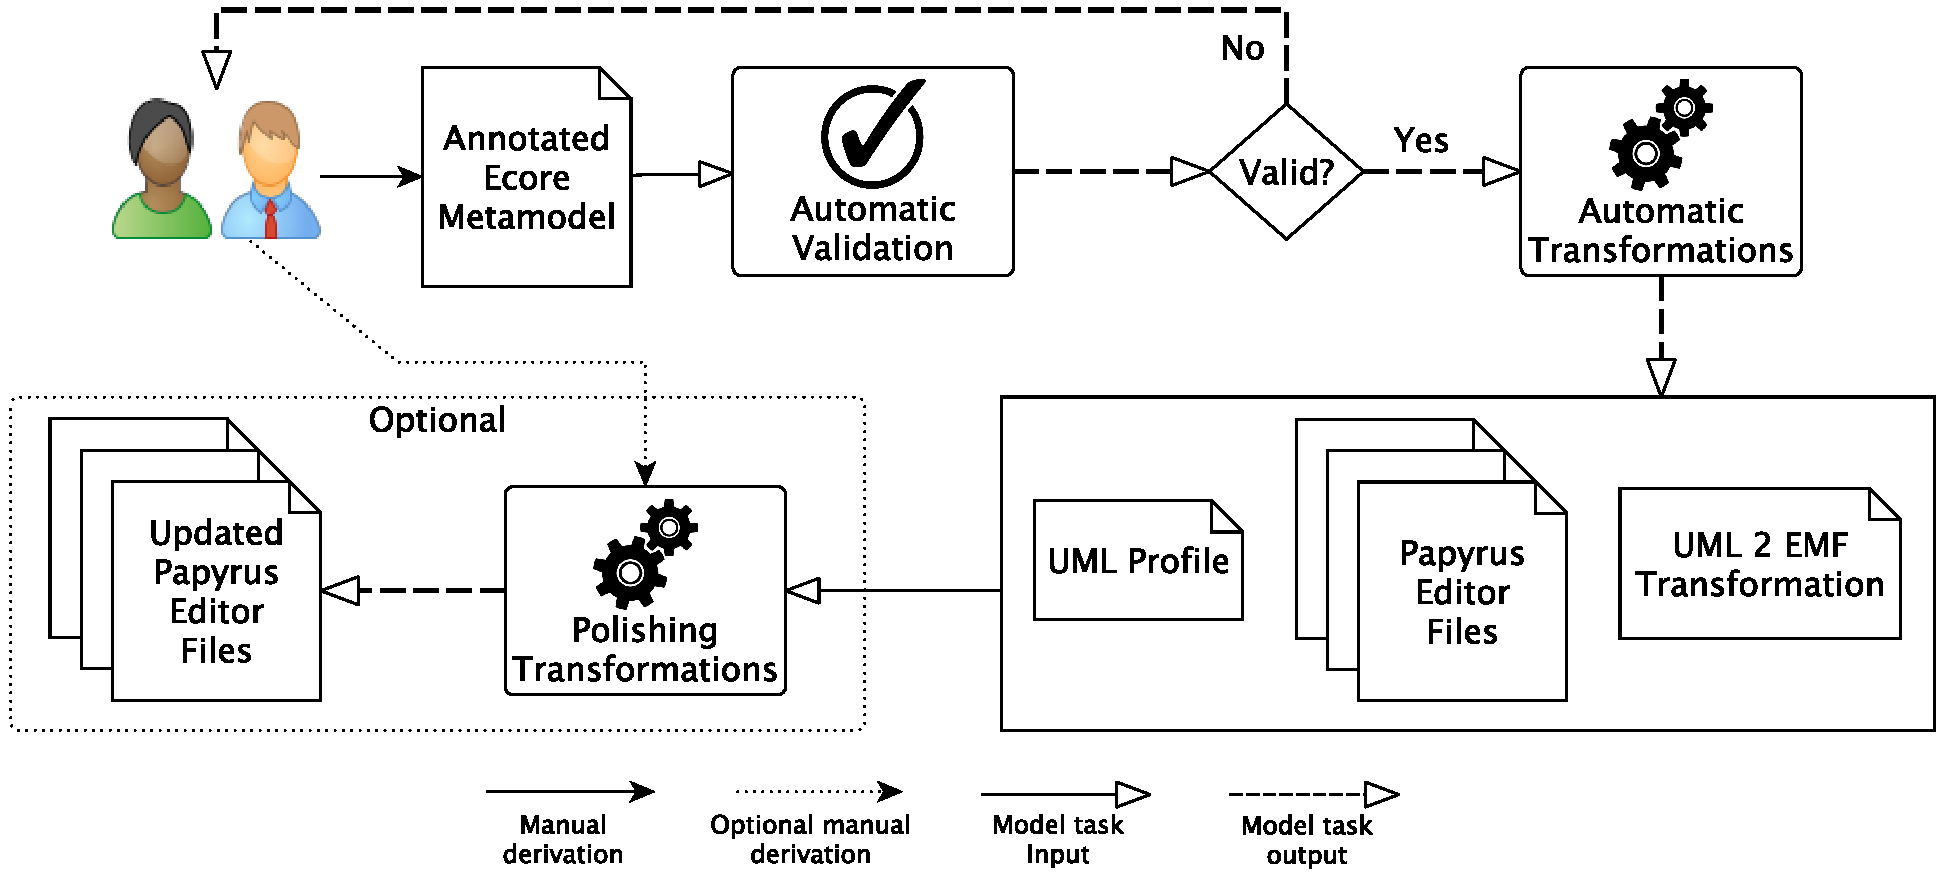
\includegraphics[width=1\textwidth]{diagrams/approachOverview.pdf}
	\caption[]{An overview of the proposed approach}
	\label{fig:approachOverview}
	\vspace{-6mm}
\end{figure}

All EClasses in the Ecore metamodel are automatically transformed into stereotypes. Stereotypes are also created from annotated EReferences (more about this below). Depending on the required graphical syntax of the stereotype (i.e., if it should be represented as a \textit{node} or as an \textit{edge} on the diagram), developers need to use the annotation on EClasses/EReferences. The approach supports the following annotations. A detailed list of all valid annotation properties is given in the Appendix. 
\begin{enumerate}[label=\arabic*.]
	\item \textbf{@Diagram} annotations are used to define diagram-specific 
	information like the name and the icon of the diagram type. This annotation 
	is always placed at the top package of the Ecore metamodel.
	\item \textbf{@Node} annotations are used to indicate the stereotypes that 
	should be instantiated as nodes in the diagrams. The UML meta-element that 
	this stereotype extends is provided through the \emph{base} property. The 
	SVG shape to be used on the canvas and the icon of the specific element in 
	the palette are specified through the \emph{shape} and \emph{icon} 
	properties, respectively.
	\item \textbf{@Edge} annotations are used to denote stereotypes that should be instantiated as edges in the diagrams. The UML meta-element extended by this stereotype is provided through the \emph{base} property. The icon of the specific element in the palette is also passed as property along with the desired style of the line. This annotation can be applied either to an EClass or to an EReference.
\end{enumerate}

Annotated Ecore metamodels are then consumed by a workflow of M2M and M2T 
transformations illustrated in Figure~\ref{fig:transformationWorkflow} and 
described in detail in Section~\ref{sec:implementation}. The transformations 
are written in the Epsilon Transformation Language (ETL)~\cite{Kolovos2008} and 
the Epsilon Generation Language (EGL)~\cite{rose2008egl} but in principle, any 
other M2M and M2T language could be used (e.g., ATL~\cite{jouault2006atl}). The 
transformations produce the UML 
profile with the appropriate OCL constraints and all the configuration models 
and files needed by Papyrus. In addition, an M2M transformation is also generated that can be used 
later by developers to transform the UML models that conform to the generated 
UML profile, back to EMF models that conform to the Ecore metamodel used as 
source. Model management programs already developed to run against model 
conforming to the EMF metamodel can be re-used.

The approach offers an optional step, that of \textit{polishing transformations}, where developers are able to write their own transformations to fine-tune the generated artefacts produced by the built-in transformations. In the following section, the proposed approach is explained via a running example.

\subsection{Running Example}
\label{sec:example}
In this example we will define and generate the UML profile and the Papyrus 
graphical editor configuration artefacts for a Simple Development Processes 
Language (SDPL) using AMIGO. We start by defining the abstract syntax of the language using 
Emfatic, a textual notation for Ecore (see 
Listing~\ref{lst:annotatedSdplEmfatic} - ignore the annotations at this point). 
A process defined in SDPL consists of \textit{Steps}, 
\textit{Tools} and \textit{Persons} participating in it. Each person is 
familiar with certain tools and can have different \textit{Role}s in steps of a 
process, while each step refers to the next step that follows using the 
\textit{next} reference.

In order to generate the UML profile and the Papyrus graphical editor we need 
to add the following concrete syntax-related annotations shown in 
Listing~\ref{lst:annotatedSdplEmfatic}:

\begin{figure}[t]
	\lstinputlisting[caption={The annotated Emfatic code that defines the 
		metamodel 
		of\\ SDPL and can be used to generate the UML profile and the 
		associated \\Papyrus 
		editor.},label={lst:annotatedSdplEmfatic},captionpos=b, 
	language=Emfatic, 
	tabsize=2, numbers=left, numbersep=5pt, numberstyle=\tiny,  
	breaklines=true]{sdplAnnotated.emf}
	
	\vspace*{-5mm}
\end{figure}

\begin{itemize}
	\item[--] \textbf{Line 2:} The name and the icon that should be used by Papyrus in the custom diagrams menus are defined using the \textit{name} and \textit{icon} properties of the \textit{@Diagram} annotation.
	\item[--] \textbf{Lines 5, 10 \& 15:} The \textit{@Node} annotation is used to define that the three concepts (i.e., Steps, Roles and Tools) should be stereotypes in the UML profile that will be represented as nodes on the diagram. The \textit{base} parameter is used to define which UML meta-element the stereotype should extend (i.e., \textit{Class}\footnote{Although profiles are meant to accommodate ``natural'' extensions to UML artefacts, sometimes is the case that generic meta-elements are used instead. For example, in the Archimate for Papyrus tool presented in Section~\ref{sec:efficiencyEvaluation}, the Use Case meta-element is used as base for the \textit{Business Service} stereotype, or Class as the base for the \textit{Business Role} stereotype. Thus, the selection of the most appropriate base element is left for the user.} in the stereotypes of this example). The shape on the canvas and the icon in the palette for each stereotype are given using the \textit{shape} and \textit{icon} annotation details.
	\item[--] \textbf{Line 20 \& 23:} The EReference \textit{familiarWith} and the \textit{Role} EClass are added in the profile as stereotypes that extend the meta-element \textit{Association} of UML. These stereotypes should be represented as links in the diagrams and thus are annotated with the \textit{@Edge} string.
	In contrast with the \textit{familiarWith EReference}, the types the 
	\textit{Roles} edge should be able to connect are not know and need to be 
	specified as properties of the annotation (i.e., \textit{source=``src''} 
	and \textit{target=``tar''}). This denotes that the source/target nodes of 
	this connector are mapped to the values of the \textit{src}/\textit{tar} 
	EReferences, respectively.
	\item{--} \textbf{NB Line 8:} The \textit{next} EReference is not required 
	to be displayed as an edge on the diagram thus it is not annotated with 
	\emph{@Edge}. However, it will be a property of the \textit{Step} 
	stereotype in the generated profile, so it can be set in the model (but it 
	will not be displayed on the diagram).
\end{itemize}


The automated M2M and M2T transformations discussed above are then executed on the Ecore file and the produced SDPL Papyrus editor is presented in Figure~\ref{fig:sdplEditor}. 

\subsection{Polishing Transformations}
This generated editor is fully functional but it can be further customised to 
fit custom user needs. For example, by default, our automatic transformations 
dictate the diagram, through the CSS file to show the stereotype name applied 
to each node. However, in this example we want to hide the stereotype names and 
display labels in red font. This can be achieved by manually amending the 
generated CSS file. However, the CSS file will be automatically overridden if 
the user regenerates the profile and the editor in the future (e.g., because of 
a change in the metamodel) . To avoid this, the user can use the -- optional 
-- CSS generation polishing transformation (\#6b in 
Figure~\ref{fig:transformationWorkflow}) shown in 
Listing~\ref{lst:cssPolishingExample}. Every time the profile and editor 
generation is executed, the polishing transformation will be called and will 
set the visibility of the stereotypes to false automatically. 

\begin{figure}[t]
	\lstinputlisting[caption={The polishing transformation for the CSS file 
	generation that\\ sets the visibility of the names of the nodes to 
	true.},label={lst:cssPolishingExample},captionpos=b, language=EGL, 
	tabsize=2, numbers=left, numbersep=5pt, numberstyle=\tiny, 
	breaklines=true]{cssPolishingExample.egl}
	
	\vspace*{-6mm}
\end{figure}

%\dk{What about inheritance? If a class is annotated as @Node and its 
%subclasses are annotation-less do they inherit the @Node annotation and its 
%details?} Thanos: No...

The EGL template in Listing~\ref{lst:cssPolishingExample} generates a CSS rule 
in lines 1-3 that sets the visibility property of the stereotypes' labels to 
false. It stores all the elements in the Ecore metamodel that are annotated as 
@Node (line 6) in a collection and iterates though them in lines 7-10. For 
each of the node stereotypes, it generates the static text 
``[appliedStereotypes~='' followed by the name of each stereotype and a comma. 
At the end it prints the curly brackets (lines 10 and 12) and the text 
``fontColor:red;'' in line 11. The resulted output that is amended 
automatically in the original CSS file by the polishing transformation is the 
one shown in Listing~\ref{lst:cssPolishingOutput}.

\begin{figure}[h]
	\vspace*{-5mm}
	\lstinputlisting[caption={The output that is amended in the original CSS 
		file using the\\ CSS polishing transformation of 
		Listing~\ref{lst:cssPolishingExample}},label={lst:cssPolishingOutput},captionpos=b,
	language=CSS, tabsize=2, numbers=left, numbersep=5pt, numberstyle=\tiny, 
	breaklines=true]{cssPolishingOutput.egl}
	\vspace*{-5mm}
\end{figure}

%Beyond providing a disciplined mechanism for customising the produced UML 
%profile and editor polishing transformations also offer an extension point for 
%future evolution of the proposed approach: user defined polishing 
%transformations developed to fulfil scenarios that we do support can be created 
%and submitted to be included in the default transformations of our approach.
%\sg{This paragraph is unclear}.

\begin{figure*}[t]
	\centering
	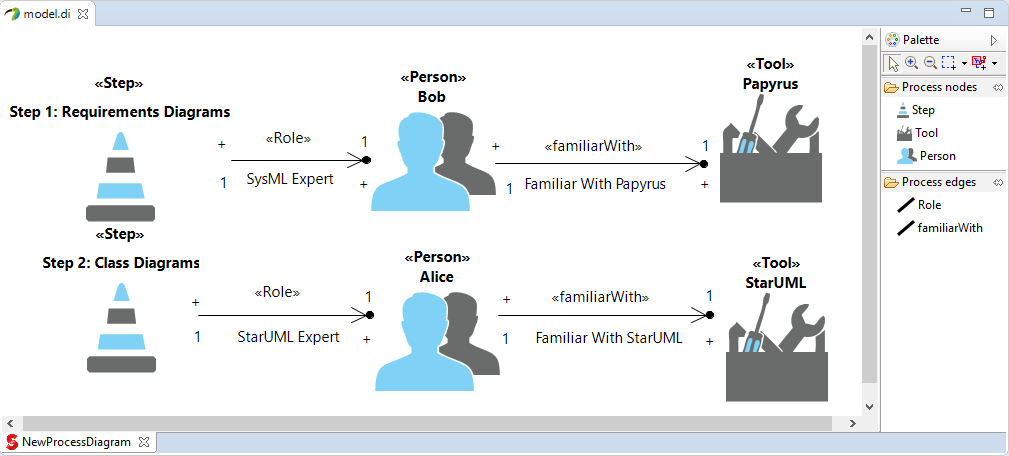
\includegraphics[width=1\textwidth]{images/sdplEditor.png}
	\caption[]{The SDPL editor for Papyrus where two steps in the software 
		development process are defined and responsible persons are attached to 
		them\\ along with the tools they are specialized on.}
	\label{fig:sdplEditor}
	
\end{figure*}